\section{General}
	\subsection{Terms and Definitions}
		\begin{table}[H]
			\centering
			\begin{tabular}{|>{\bfseries}p{0.3\linewidth}|p{0.65\linewidth}|}
				 \hline
				 CPU bound
				 	& Algorithms that use bursts of CPU time.\\
				 \hline
				 I/O bound  
				 	& Algorithms that spend much time waiting for I/O\\
				 \hline		
				 Row major order  
				 	& In multidimensional arrays row elements are stored next to each other (C/C++, Pascal\ldots)\\
				 \hline
				 Column major order  
				 	& In multidimensional arrays column elements are stored next to each other (Matlab, Fortran, Octave\ldots)\\
				\hline
			\end{tabular}
		\end{table}
	
	\subsection{Elements of an FPGA \weekMaehne{1}}
		\begin{multicols}{2}
			\textbf{Look-Up-Table (LUT:)} Any logic function can be expressed as a sum of products. \\
			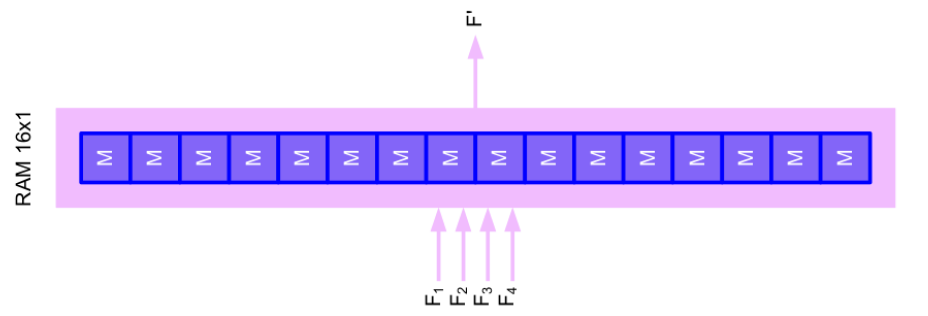
\includegraphics[width=0.4\textwidth]{./pictures/LUT.png} \\
			\textbf{Basic Logic Element (BLE) or Logic Cell:} \\
			\includegraphics[width=0.4\textwidth]{./pictures/BLE.png} \\
			\textbf{Switch Box (SB), Connection Box (CB):} \\
			\includegraphics[width=0.4\textwidth]{./pictures/SB.png} \\
			\textbf{Configurable Logic Block (CLB):} \\
			\includegraphics[width=0.4\textwidth]{./pictures/CLB.png} \\ 		
			\textbf{Input/Output block (IOB):}  \\
			\includegraphics[width=0.4\textwidth]{./pictures/IOB.png} \\
			\textbf{Dedicated Blocks (DBs):} \\
			Configurable specialized blocks implementing commonly needed functionality efficiently
			\begin{compactitem}
				\item Block SRAM
				\item Digital Clock Manager (DCM), DLL, PLL
				\item Multiplier
				\item DSP block
				\item Complete CPU cores
			\end{compactitem}
		\end{multicols}
		
	